\documentclass[10pt,pdf,hyperref={unicode}, dvipsnames]{beamer}
\usepackage[english,russian]{babel}
% \usepackage[T2A,T1]{fontenc}
\usepackage[utf8]{inputenc}
\usepackage{tikz}
\usepackage[unicode]{hyperref}
\usepackage{pgfplots,standalone}
% \usepackage{lmodern}
\pgfplotsset{compat=newest} 
\usetikzlibrary{%
    decorations.pathreplacing,%
    decorations.pathmorphing,%
    patterns,%
    angles,%
    quotes,%
    calc, %
    3d, %
    backgrounds, %
    positioning%
}

% Стиль презентации
\usetheme{Warsaw}

% \setbeamercolor{frametitle right}{fg=white,bg=Brown!85}
% \setbeamercolor{frametitle}{fg=white,bg=Brown!85}
\setbeamercolor{frametitle right}{fg=white,bg=black!85}
\setbeamercolor{frametitle}{fg=white,bg=black!85}

\setbeamertemplate{headline}{}
\setbeamertemplate{footline}{}
\let\Tiny=\tiny % решает проблему со шрифтами в TexLive
\setbeamertemplate
	{footline}{
		\color{black!40!white}
		\quad\hfill
		\insertframenumber/\inserttotalframenumber
		\hfill\vspace{1em}\quad
	} 

\setbeamertemplate{navigation symbols}{}

\beamersetrightmargin{0.5cm} 
\beamersetleftmargin{0.5cm}

\setbeamertemplate{enumerate item}{
	\usebeamercolor[bg]{item projected}
	\raisebox{1pt}{\colorbox{bg}{\color{fg}\footnotesize\bf\insertenumlabel}}%
}
\setbeamercolor{item projected}{bg=black,fg=white}

\setbeamertemplate{itemize item}{%
	\usebeamercolor[bg]{item projected}%
	\raisebox{1pt}{{\color{bg}\footnotesize$\bf\square$}}%
}
\setbeamercolor{item projected}{bg=black,fg=white}
\setbeamercolor{title}{bg=black,fg=white}
\newcommand\frametitless[1]{\subsection{#1}\frametitle{#1}}
\usepackage{booktabs, setspace}
\newcommand{\tabitem}{~~\llap{\textbullet}~~}
\setbeamertemplate{caption}{\raggedright\insertcaption\par}
\title[]{Твердотельный лазер на керамике с волоконно-лазерной накачкой}

\author{%
	Геликонова В.Г., %
	Платонова М.В., %
	Сарафанов Ф.Г. %
}

\institute{Радиофизический факультет ННГУ, 420 группа}

\date{Нижний Новгород, 2017}

\begin{document}  

%%%%%%%%%%%%%%%%%%%%%%%%%%%%%%%%%%%%%%%%%%%%%%%%%%%%%%%%%%%%%
\begin{frame}[plain]
	\centering
	\vspace{2cm}
	\begin{beamercolorbox}[sep=8pt,center]{title}
		\bf\usebeamerfont{title}\inserttitle
	\end{beamercolorbox}
	\vspace{0.5cm}
	\normalsize \textbf{Работу выполнили:}\\
	\large\insertauthor\\ 
	\vspace{0.5cm}
	\normalsize{\textbf{Научный руководитель:}\\}
	\large{Антипов О.Л.}
	\vfill
	\small{Нижний Новгород -- 2017}
\end{frame}
%%%%%%%%%%%%%%%%%%%%%%%%%%%%%%%%%%%%%%%%%%%%%%%%%%%%%%%%%%%%%
% \begin{frame}[t]
%   \frametitle{Содержание}
%   \tableofcontents
% \end{frame}
%%%%%%%%%%%%%%%%%%%%%%%%%%%%%%%%%%%%%%%%%%%%%%%%%%%%%%%%%%%%%
\section{Цели работы}
\begin{frame}[t]
	\frametitle{Цели работы}
	% \textbf{Цели}\\
	\vfill
\begin{spacing}{1}
	\begin{enumerate}
		\item Ознакомиться с принципами работы  лазера
		\item Измерить мощность волоконного и твердотельного лазеров
		\item Поучаствовать в эксперименте по созданию лазера и измерению его параметров	
	\end{enumerate}
\end{spacing}
	\vfill
\end{frame}
%%%%%%%%%%%%%%%%%%%%%%%%%%%%%%%%%%%%%%%%%%%%%%%%%%%%%%%%%%%%%
\section{Теоретическая часть}
\begin{frame}[t]
	\frametitless{Виды переходов электронов между уровнями энергии}
	\begin{enumerate}
		\item \textbf{Спонтанное излучение}
	\end{enumerate}
	\begin{center}
		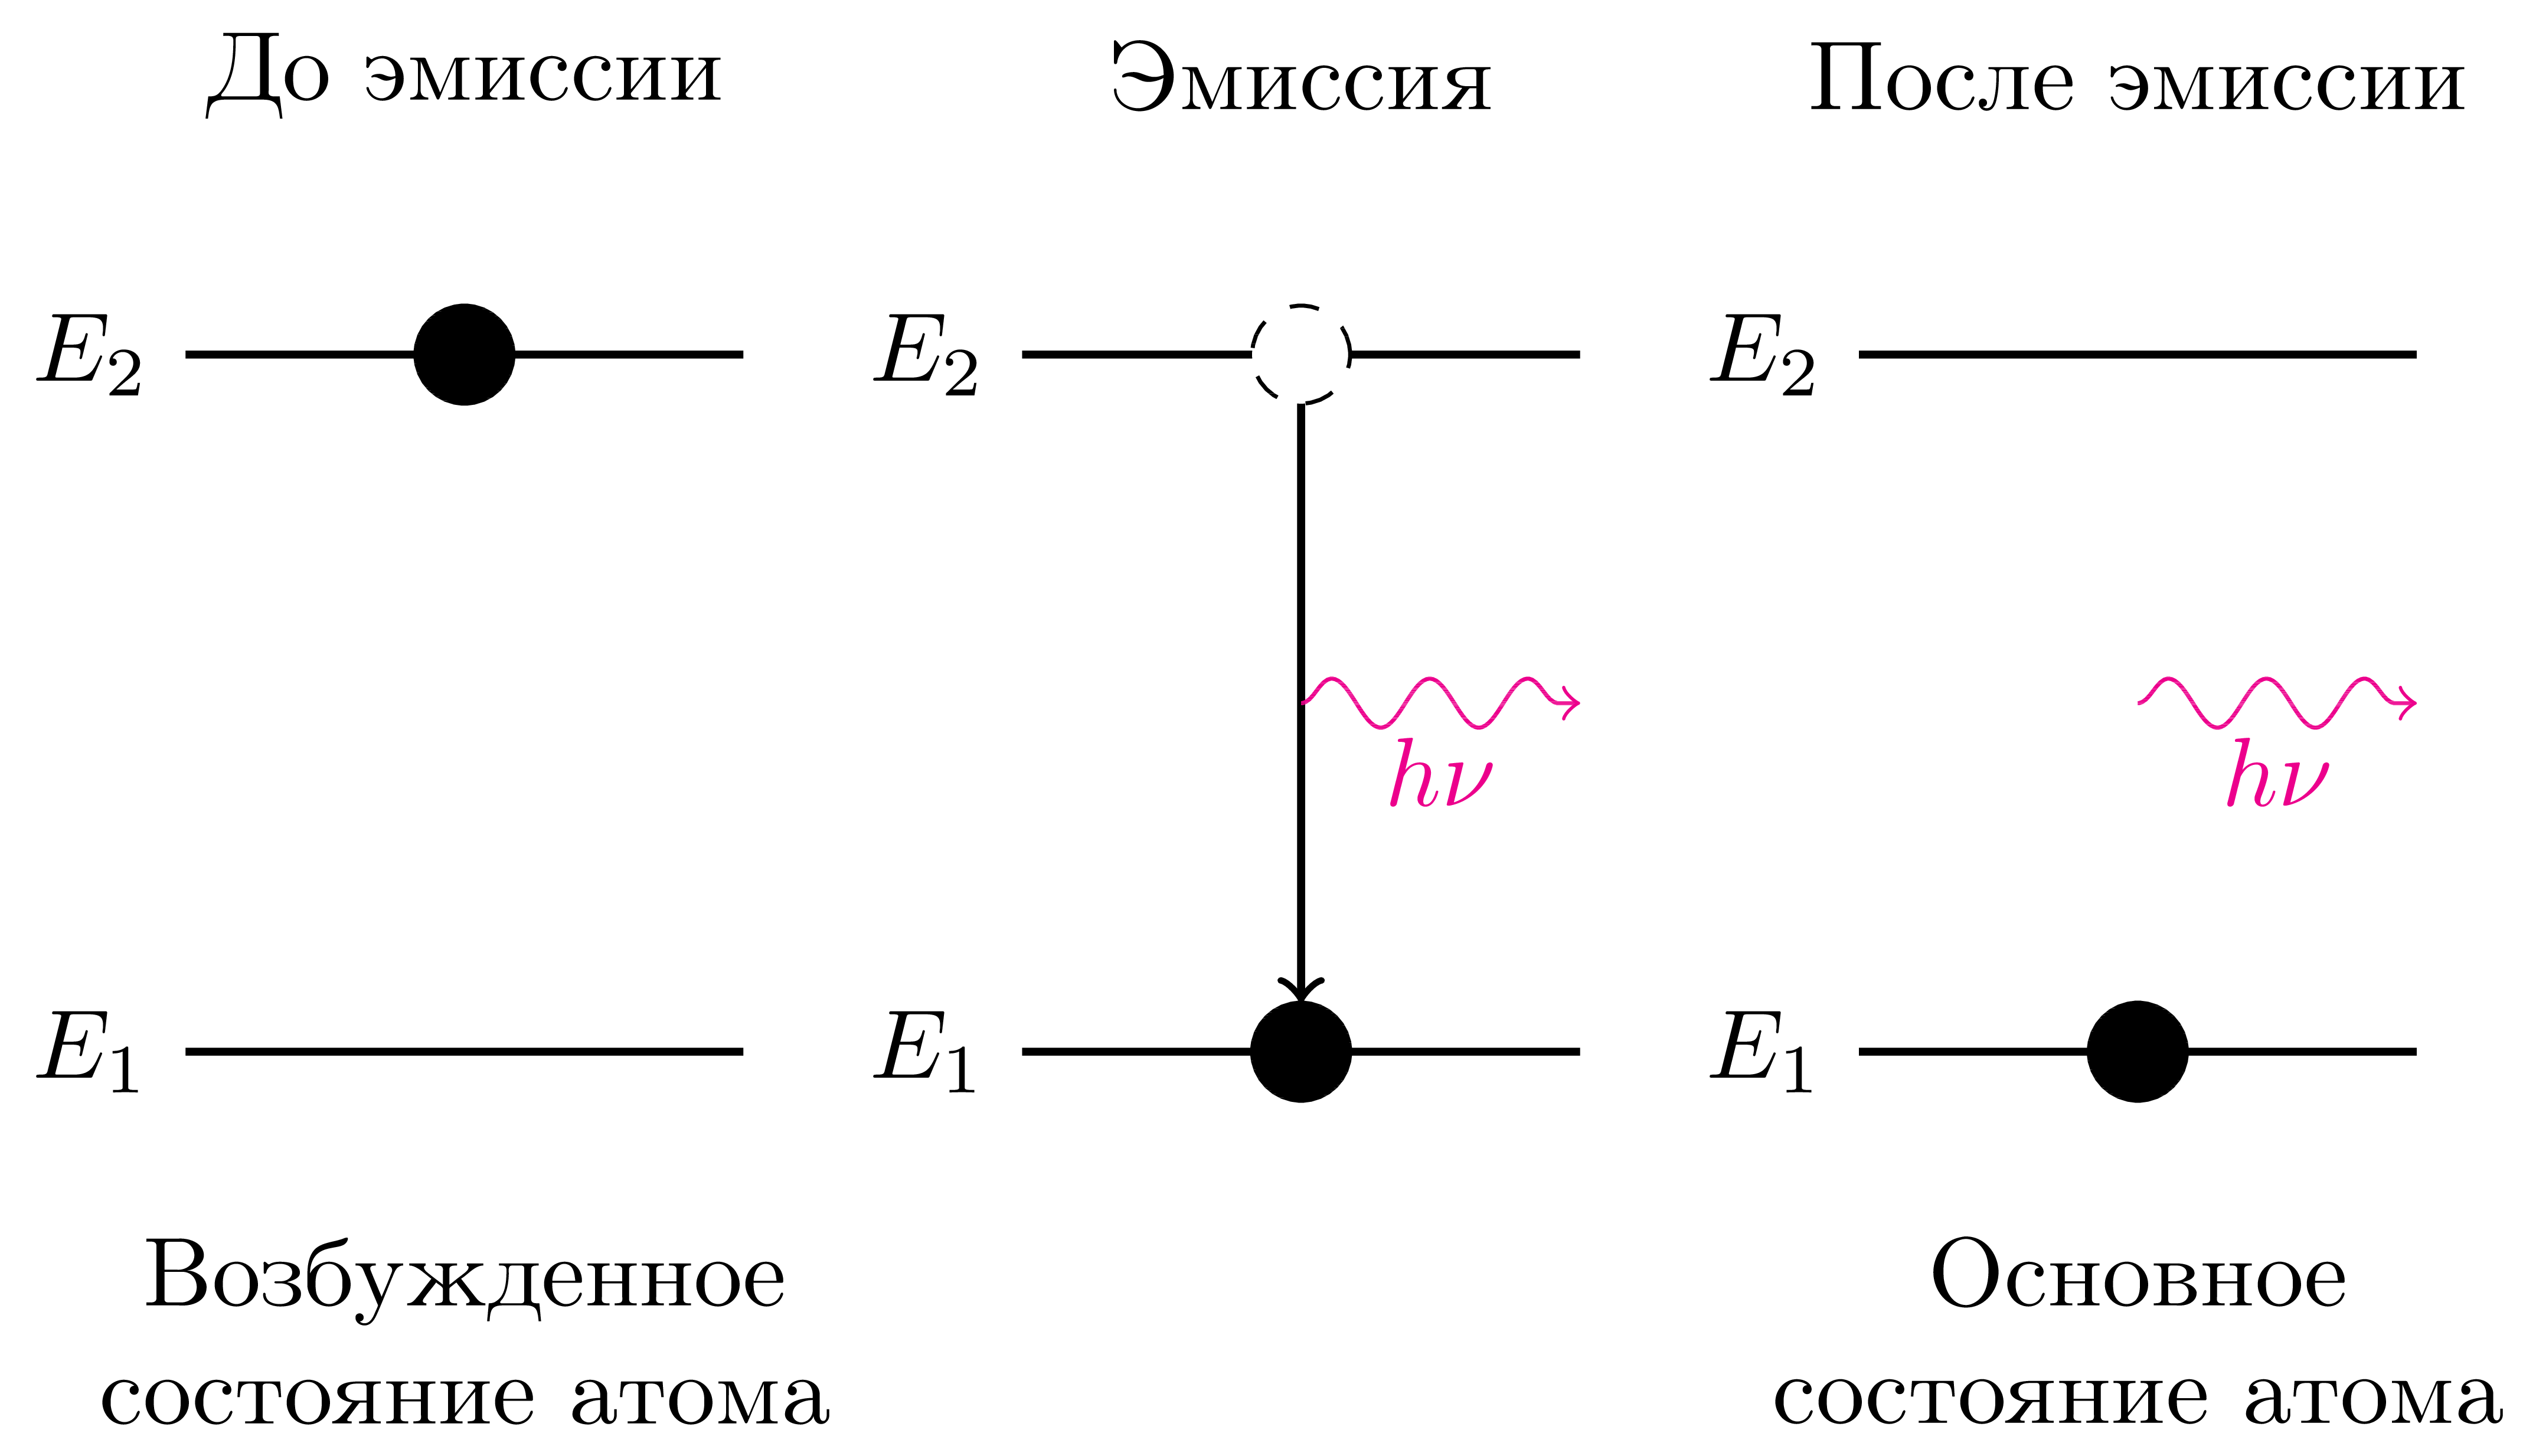
\includegraphics[]{images/spont}
	\end{center}
\end{frame}
%%%%%%%%%%%%%%%%%%%%%%%%%%%%%%%%%%%%%%%%%%%%%%%%%%%%%%%%%%%%%
\begin{frame}[t]
	\frametitless{Виды переходов электронов между уровнями энергии}
	\begin{enumerate}
		\setcounter{enumi}{1}	
		\item \textbf{Вынужденное излучение}
	\end{enumerate}
	\begin{center}
		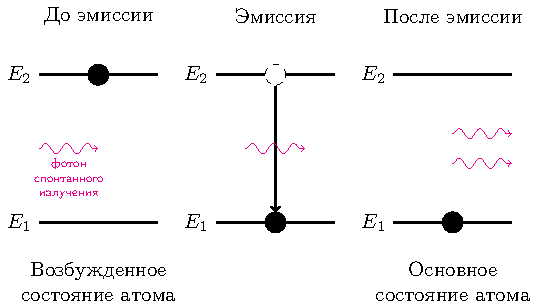
\includegraphics[]{images/forced}
	\end{center}
\end{frame}
%%%%%%%%%%%%%%%%%%%%%%%%%%%%%%%%%%%%%%%%%%%%%%%%%%%%%%%%%%%%%
\begin{frame}[t] 
	\frametitless{Устройство лазера}
	\textbf{Лазер} [\textbf{L}ight \textbf{A}mplification by \textbf{S}timulated \textbf{E}mition of \textbf{R}adiation ] -- устройство, усиливающее свет посредством вынужденного излучения.

	\begin{figure}[h]
		\centering
		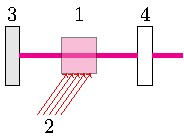
\includegraphics[width=0.3\textwidth]{images/las1}
	\end{figure}	




	Основные составляющие:
		\vspace{1em}
	\begin{columns}[t]
		\begin{column}{0.45\textwidth}
			% \begin{enumerate}
				\textbf{1} -- Активная (рабочая) среда\\
				\textbf{2} -- Система накачки (источник энергии)
			% \end{enumerate}
		\end{column}
		\begin{column}{0.45\textwidth}
			% \begin{enumerate}
				% \setcounter{enumi}{2}		
				\textbf{3} -- Непрозрачное зеркало\\
				\textbf{4} -- Полупрозрачное зеркало
			% \end{enumerate}
		\end{column}
	\end{columns}
\end{frame}

%%%%%%%%%%%%%%%%%%%%%%%%%%%%%%%%%%%%%%%%%%%%%%%%%%%%%%%%%%%%%
\begin{frame}[t]
	\frametitless{Накачка}
	\textbf{Накачка} -- процесс создания инверсии населенностей в активной среде 

	\vspace{1em}
	\textbf{Инверсия населенностей} -- состояние вещества, при  котором на высоком рабочем уровне энергии находится большее количество электронов, чем на нижнем

	\vspace{1em}
	Виды накачки: 
	\begin{enumerate}
		\item оптическая – за счет энергии света
		\item электрическая – накачка электрическим током
		\item химическая – с использованием энергии химических реакций
	\end{enumerate}
\end{frame}
%%%%%%%%%%%%%%%%%%%%%%%%%%%%%%%%%%%%%%%%%%%%%%%%%%%%%%%%%%%%%
\begin{frame}[t]
	\frametitless{Активные среды и энергетические уровни}

	\begin{columns}
		\begin{column}{0.49\textwidth}
			\begin{figure}[h]
				\centering
				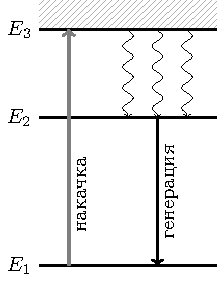
\includegraphics[]{images/3nd}
				\caption{3-уровневая среда}
			\end{figure}	
		\end{column}
		\begin{column}{0.49\textwidth}
			\begin{figure}[h]
				\centering
				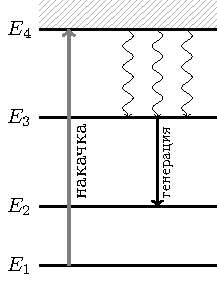
\includegraphics[]{images/4nd}
				\caption{4-уровневая среда}
			\end{figure}	
		\end{column}
	\end{columns}
	\vspace{1em}
	В лазере сначала происходит спонтанный переход, фотоны от него создают вынужденное излучение других фотонов, когерентных первоначальным, таким образом возникает фотонная лавина, усиливающаяся в резонаторе

\end{frame}
%%%%%%%%%%%%%%%%%%%%%%%%%%%%%%%%%%%%%%%%%%%%%%%%%%%%%%%%%%%%%
\begin{frame}[t]
	\frametitless{Резонатор}

	\vfill
	\begin{figure}[h]
		\centering
		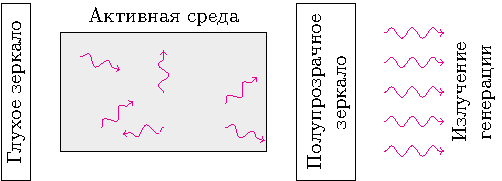
\includegraphics[]{images/resonator}
		\caption{Простейший резонатор}
	\end{figure}	
	\vfill 
	В простейшем случае представляет собой два зеркала, установленных друг напротив друга, одно из которых полупрозрачное -- через него луч лазера частично выходит из резонатора
	% Для увеличения мощности выходного излучения применяют модуляцию добротности – уменьшают пропускную способность непрозрачного зеркала
\end{frame}
%%%%%%%%%%%%%%%%%%%%%%%%%%%%%%%%%%%%%%%%%%%%%%%%%%%%%%%%%%%%%
% \begin{frame}[t]
% 	\frametitless{Модуляция добротности}
% 	\textbf{Модуляция добротности} -- метод, применяемый для получения импульсного режима работы лазера

% 	\vspace{1em}
% 	Некоторые методы модуляции:

% 	\begin{enumerate}
% 		\item Вращающееся зеркало
% 		\item Ячейки Поккельса (электрооптические затворы)
% 		\item Насыщающийся поглотитель
% 		\item Акустооптическая модуляция

% 	\end{enumerate}
% 	\begin{columns}
% 		\begin{column}{0.3\textwidth}
% 			\begin{figure}[h]
% 				\centering
% 				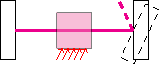
\includegraphics[]{images/rot_flip}
% 				% \caption{3-уровневая среда}
% 			\end{figure}	
% 		\end{column}
% 		\begin{column}{0.3\textwidth}
% 			\begin{figure}[h]
% 				\centering
% 				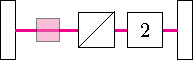
\includegraphics[]{images/pockels_cell}
% 				% \caption{4-уровневая среда}
% 			\end{figure}	
% 		\end{column}
% 		\begin{column}{0.3\textwidth}
% 			\begin{figure}[h]
% 				\centering
% 				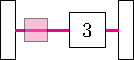
\includegraphics[]{images/pogl}
% 				% \caption{4-уровневая среда}
% 			\end{figure}	
% 		\end{column}		
% 	\end{columns}
% 		% Основная идея метода состоит в том, что во время накачки намеренно «ухудшают» свойства оптического резонатора, не давая, таким образом, лазеру излучать.

% 		% Благодаря этому мощность не расходуется на излучение и удаётся получить высокий уровень инверсной населённости энергетических уровней активной среды. 

% 		% Далее свойства резонатора быстро «улучшают», и вся накопленная энергия реализуется в виде короткого, мощного импульса.	
% \end{frame}
% %%%%%%%%%%%%%%%%%%%%%%%%%%%%%%%%%%%%%%%%%%%%%%%%%%%%%%%%%%%%%
% \begin{frame}[t]
% 	\frametitless{Акустооптическая модуляция добротности}
% 			\begin{figure}[h]
% 				\centering
% 				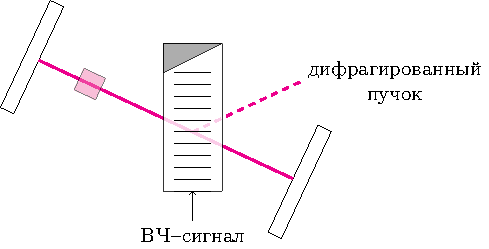
\includegraphics[]{images/aom}
% 				% \caption{4-уровневая среда}
% 			\end{figure}	
% Акустооптический модулятор представляет собой участок оптически про­зрачной среды, в котором возбуждается бегущая ультразвуковая волна.
% \\~\\
% Из-за наличия фотоупругого эффекта среду можно рассматривать как фазовую дифракционную решетку, на которой часть светового пучка в лазере дифрагирует и выходит из лазера, ухудшая добротность.
% \end{frame}



%%%%%%%%%%%%%%%%%%%%%%%%%%%%%%%%%%%%%%%%%%%%%%%%%%%%%%%%%%%%% 
\begin{frame}[t]
	\frametitless{Моды резонатора}
	\vfill
	\begin{columns}
		\begin{column}{0.49\textwidth}
				\textbf{Мода резонатора} может трактоваться как структура поля, в продольном или поперечном направлениях
				\vspace{1em}

			% \textbf{Поперечные моды} --
			 % обобщение			продольных,
			 % определяются
			% набором частот и
			% распределением поля в пучке
			% (структура поля в поперечном направлении)
				% \vspace{1em}

			\textbf{Основная мода} -- мода,
			имеющая наименьшую расходимость
% \vspace{1em}
% 			В простых плоскозеркальных
% 			резонаторах остаются только моды,
% 			для которых расстояние между
% 			зеркалами:

% 			\begin{equation*}
% 			L= q\frac{\lambda}{2}
% 			\end{equation*}
% 			(q – порядок моды)	
		\end{column}
		\begin{column}{0.49\textwidth}
			\begin{figure}[h]
				\centering
				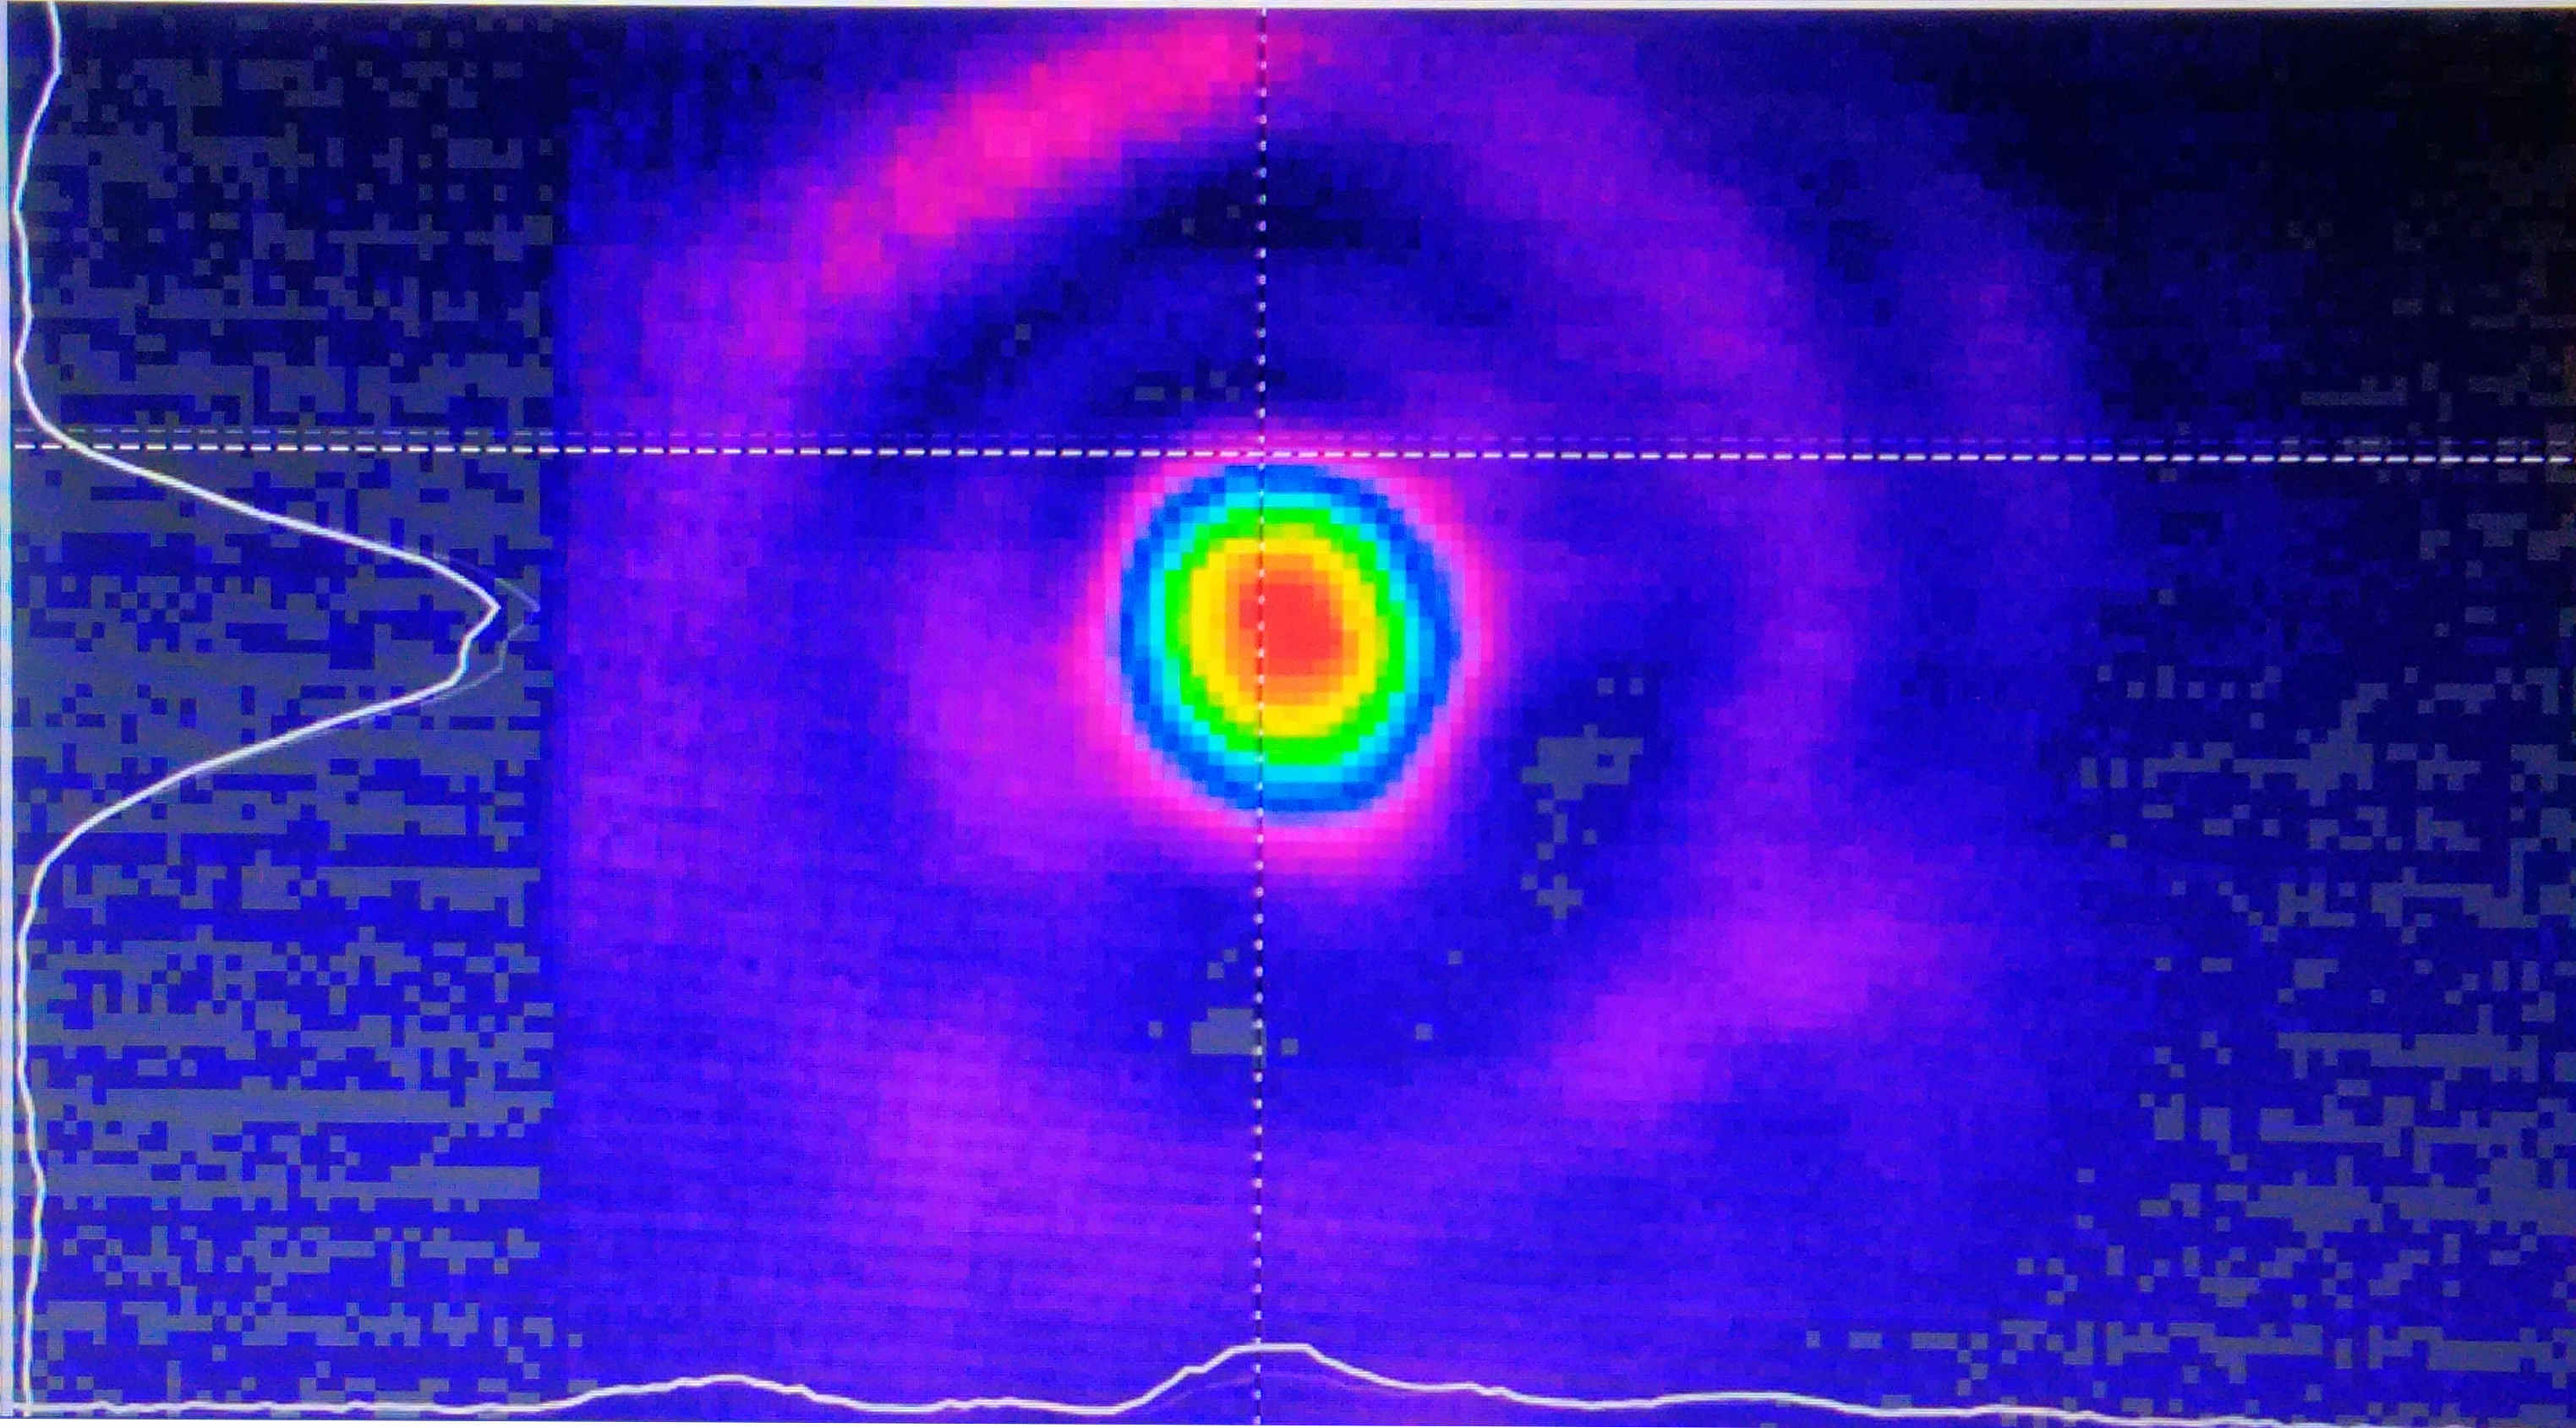
\includegraphics[width=\textwidth]{photo/light}
				\caption{Основная поперечная мода лазера на керамике}
			\end{figure}	
		\end{column}
	\end{columns}	
	\vfill
\end{frame}
%%%%%%%%%%%%%%%%%%%%%%%%%%%%%%%%%%%%%%%%%%%%%%%%%%%%%%%%%%%%%
\begin{frame}[t]
	\frametitless{Некоторые виды лазеров}
	% \vfill
	\vspace{-1em}

	\begin{columns}
		\begin{column}{0.3\textwidth}
			\begin{figure}[h]
				\centering
				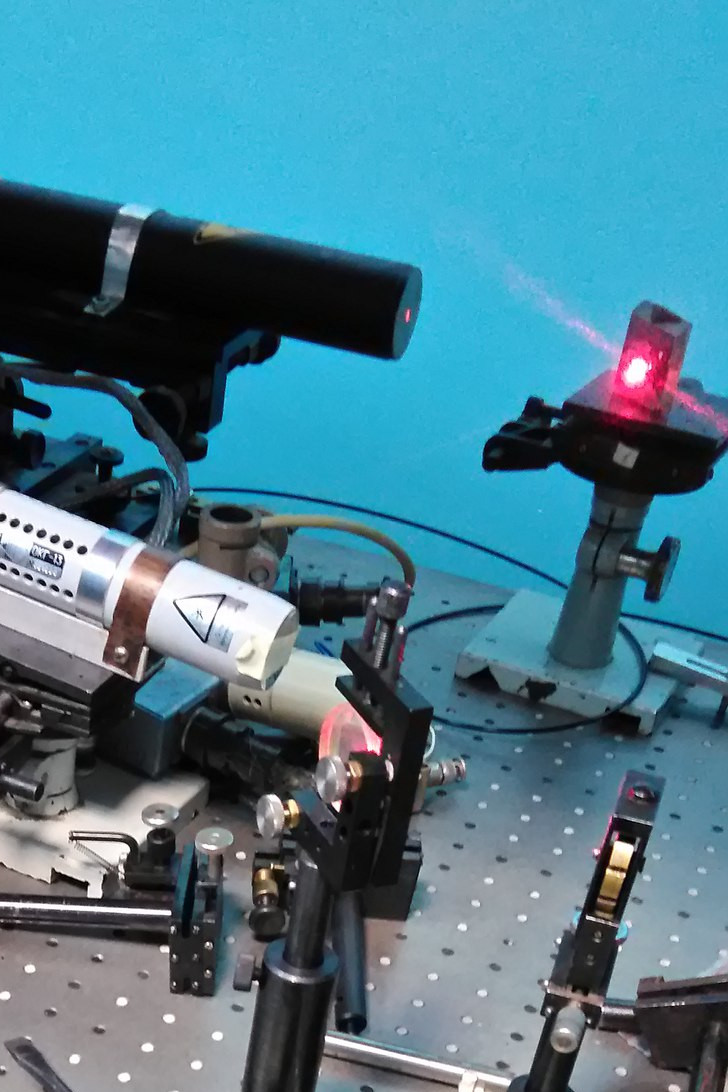
\includegraphics[width=0.8\textwidth]{photo/las_g}
				\caption{Газовый лазер}
			\end{figure}	
		\end{column}
		\begin{column}{0.3\textwidth}
			\begin{figure}[h]
				\centering
				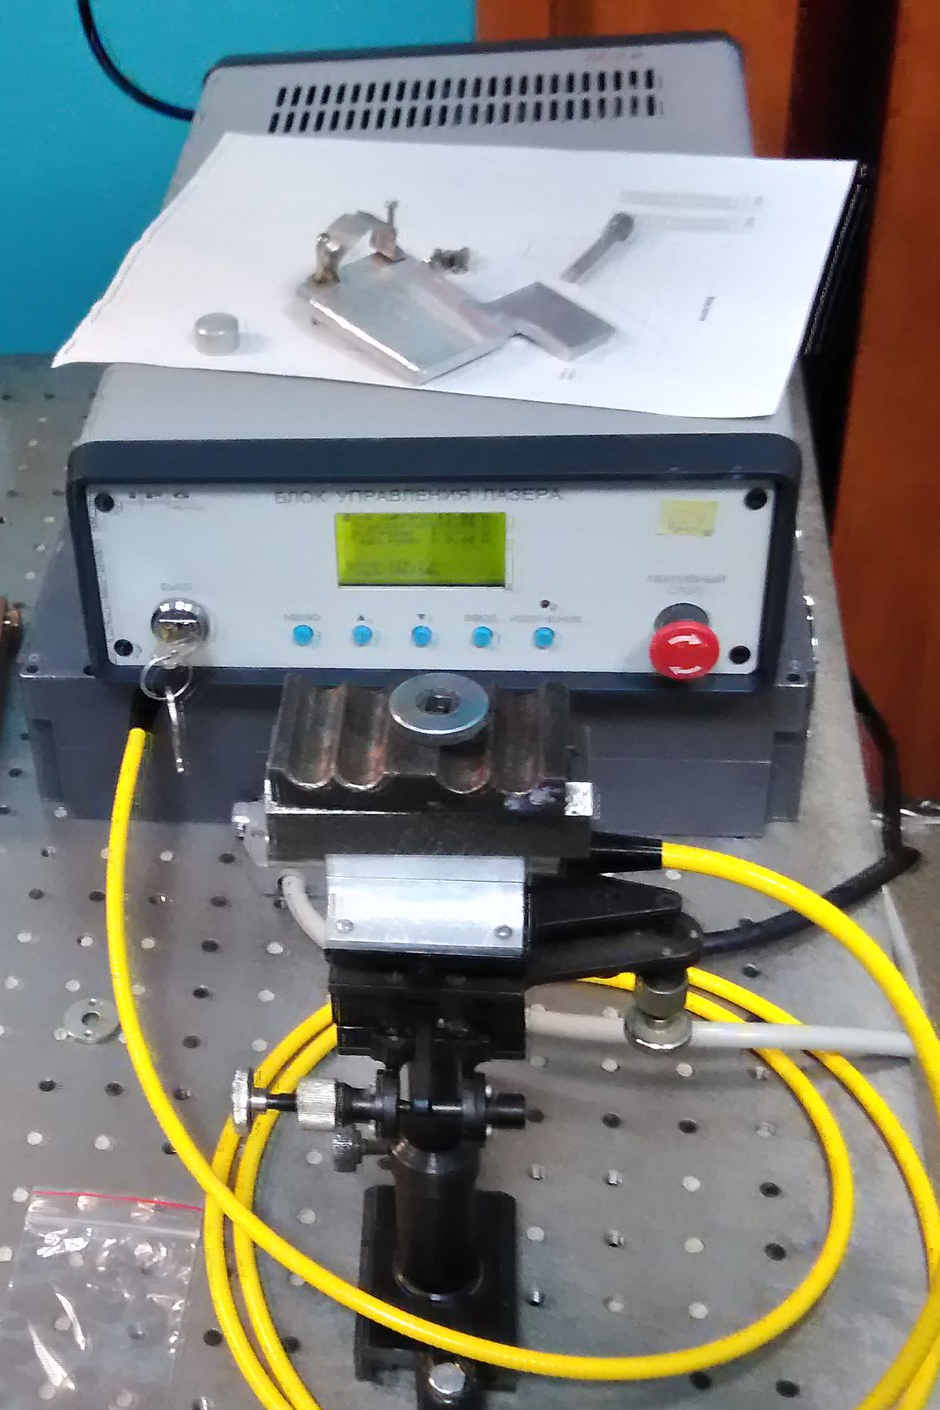
\includegraphics[width=0.8\textwidth]{photo/las_f}
				\caption{Волоконный лазер}
			\end{figure}	
		\end{column}
		\begin{column}{0.3\textwidth}
			\begin{figure}[h]
				\centering
				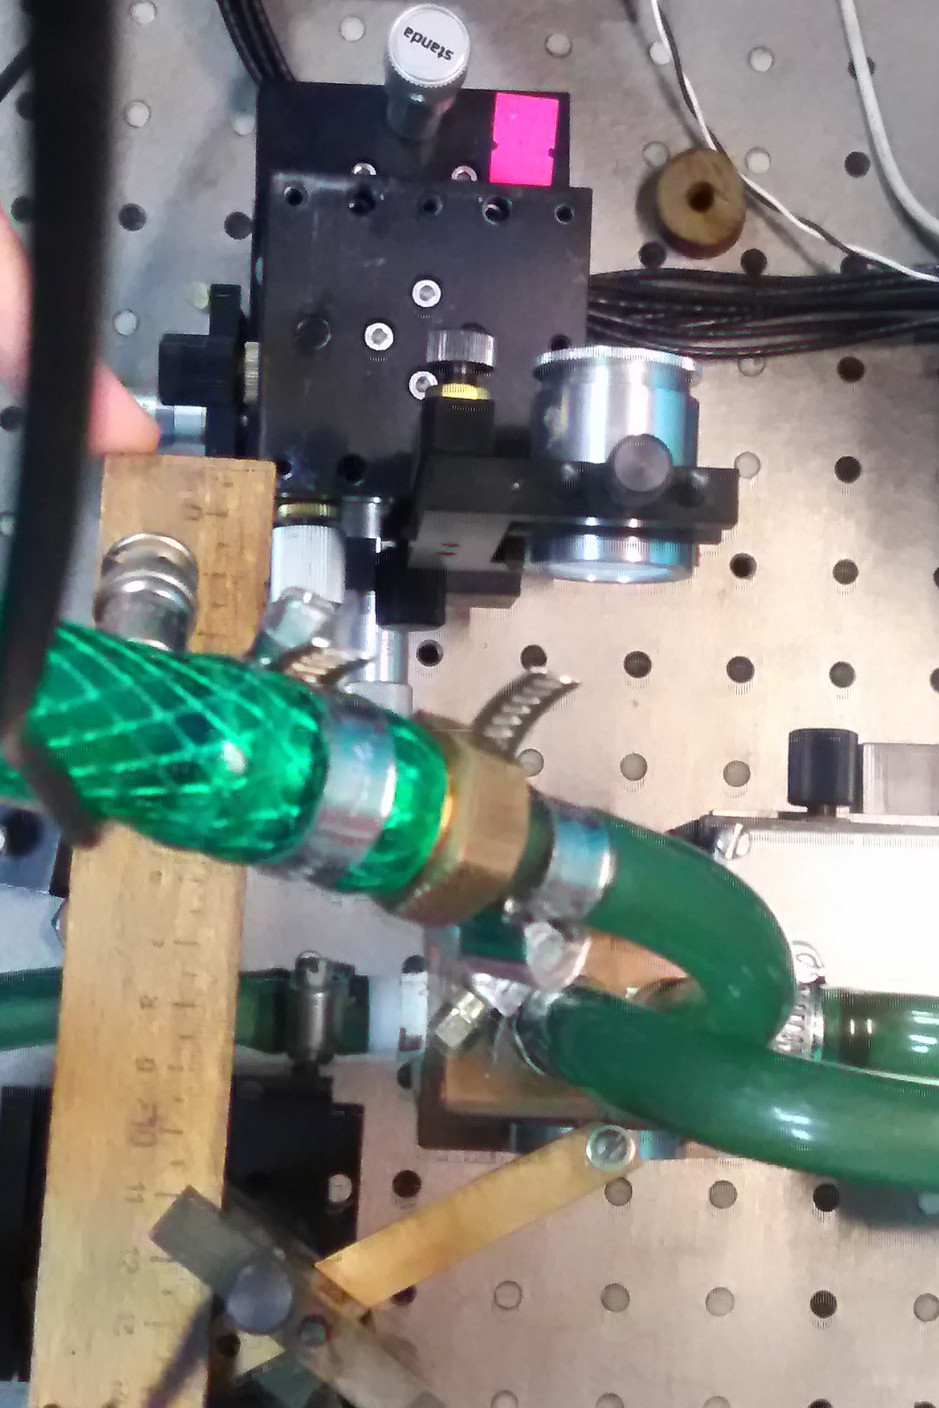
\includegraphics[width=0.8\textwidth]{photo/las_s}
				\caption{Лазер на керамике}
			\end{figure}	
		\end{column}		
	\end{columns}
	\begin{center}
  \begin{tabular}{*{4}{l}}
    \toprule
    Вид лазера & Рабочая среда & Длина волны & Мощность \\
    \midrule
    газовый & газ & 633 нм & 5  мВт\\
    \midrule
    волоконный & волокно & 1670 нм & 40 Вт\\
    \midrule
    твердотельный & кристалл/керамика & 2066 нм & 10 Вт\\
    \bottomrule
  \end{tabular}		
	\end{center}
	%\vspace{-1em}	
% \vfill
\end{frame}
%%%%%%%%%%%%%%%%%%%%%%%%%%%%%%%%%%%%%%%%%%%%%%%%%%%%%%%%%%%%% 
\begin{frame}
	\frametitless{Схема установки}
	\begin{figure}[tb]
		\centering
		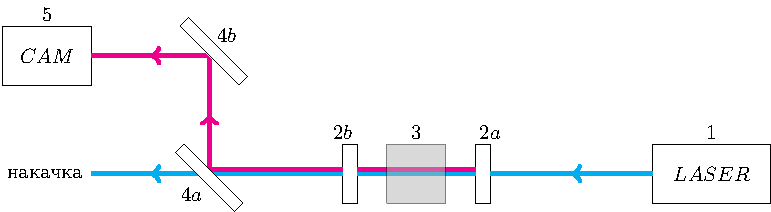
\includegraphics[width=1\textwidth]{images/chem}
	\end{figure}
	\vspace{1cm}
	\begin{columns}
		\begin{column}{0.4\textwidth}
			\textbf{1} -- волоконный лазер накачки\\ 
			\textbf{2a, 2b} -- резонатор\\
			% \textbf{2a, 2b} -- зеркала резонатора\\
			\textbf{3} -- активная среда
		\end{column}
		% \hspace{1.6cm}
		\begin{column}{0.4\textwidth}
			\textbf{4a} -- диэлектрическое зеркало\\
			\textbf{4b} -- зеркало\\
			\textbf{5} -- камера
		\end{column}
	\end{columns}
\end{frame}
%%%%%%%%%%%%%%%%%%%%%%%%%%%%%%%%%%%%%%%%%%%%%%%%%%%%%%%%%%%%% 
\begin{frame}[t]
	\frametitless{Диэлектрическое зеркало}
	\begin{columns}
		\begin{column}{0.49\textwidth}
			\begin{figure}[h]
				\centering
				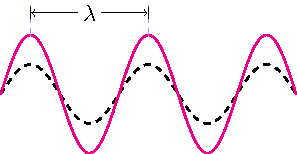
\includegraphics[]{images/interf}
				\caption{Конструктивная интерференция}
			\end{figure}	
			\begin{figure}[h]
				\centering
				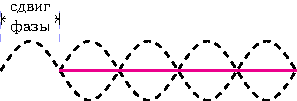
\includegraphics[]{images/interf2}
				\caption{Деструктивная интерференция}
			\end{figure}			
		\end{column}
		\begin{column}{0.49\textwidth}
			\begin{figure}[h]
				\centering
				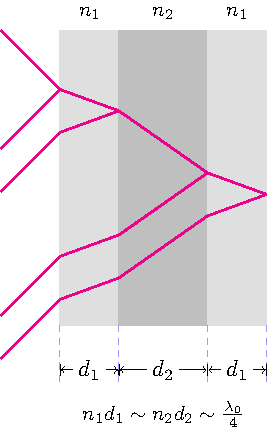
\includegraphics[]{images/df}
				% \caption{4-уровневая среда}
			\end{figure}	
		\end{column}
	\end{columns}	
\end{frame}
% Диэлектрическое зеркало представляет собой пачку слоев с чередующимся показателем преломления. 

% Толщина слоев подобрана таким образом, чтобы для избранной длины волны лабмда_0 оптический путь волны в слое был пропорционален половине длины волны.

% Отраженная часть пучка и преломленная в зеркале интерферируют. Для избранной длины волны интерференция конструктивная -- зеркало отражает, для всех остальных деструктивная - отражение ухудшается по мере удаления от длины волны ламбда 0 или вообще исчезает.
%%%%%%%%%%%%%%%%%%%%%%%%%%%%%%%%%%%%%%%%%%%%%%%%%%%%%%%%%%%%% 
\begin{frame}[t]
	\frametitless{Волоконный лазер}
% В качестве активной среды выступает волоконный световод, легированный добавками.
% \\~\\
% Оптический резонатор обычно реализуется из решеток Брэгга (структура волокна с модулированным $n$)
	% \vfill
	% \begin{columns}[c]
		% \begin{column}{0.7\textwidth}
			\begin{figure}[tb]
				\centering
				\includegraphics%[width=1\textwidth]
				{images/fil}
			\end{figure}
		% \end{column}
		% \hspace{1.6cm}
	% 	\begin{column}{0.3\textwidth}
	% 		\begin{figure}[tb]
	% 			\centering
	% 			\includegraphics[width=1\textwidth]
	% 			{photo/light.jpg}
	% 		\end{figure}
	% 	\end{column}
	% \end{columns}	
	
	% \vfill
		\vspace{1cm}
	\begin{columns}
		\begin{column}{0.4\textwidth}
			\textbf{1} -- активная среда (легированное волокно)\\ 
			\textbf{2} -- волновод накачки\\
			\textbf{3} -- внешняя оболочка
		\end{column} 
		% \hspace{1.6cm}
		\begin{column}{0.4\textwidth}
			\textbf{4} -- излучение накачки\\
			\textbf{5} -- излучение генерации\\
			\textbf{6} -- волоконная брэгговская решетка\\
			\textbf{7} -- накачка (диодный лазер)%\\
			% \textbf{5} -- камера
		\end{column}
	\end{columns}
\end{frame}
%%%%%%%%%%%%%%%%%%%%%%%%%%%%%%%%%%%%%%%%%%%%%%%%%%%%%%%%%%%%% 
\begin{frame}[t] 
	\frametitless{Зависимость излучения волоконного лазера от тока}
		\begin{figure}[tb]
		\centering
		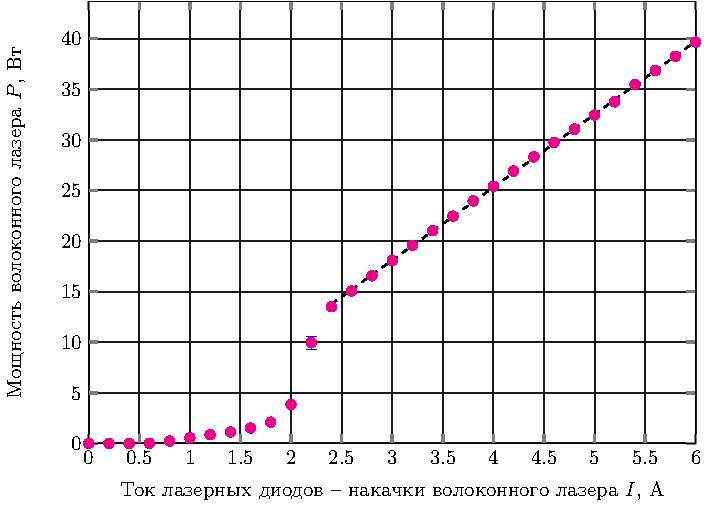
\includegraphics[width=0.9\textwidth]{img/PI}
	\end{figure}
\end{frame}
%%%%%%%%%%%%%%%%%%%%%%%%%%%%%%%%%%%%%%%%%%%%%%%%%%%%%%%%%%%%% 
\begin{frame}[t]
	\frametitless{Лазер на керамике}
	
	\begin{columns}
		\begin{column}{0.63\textwidth}
			\begin{figure}[tb]
				\centering
				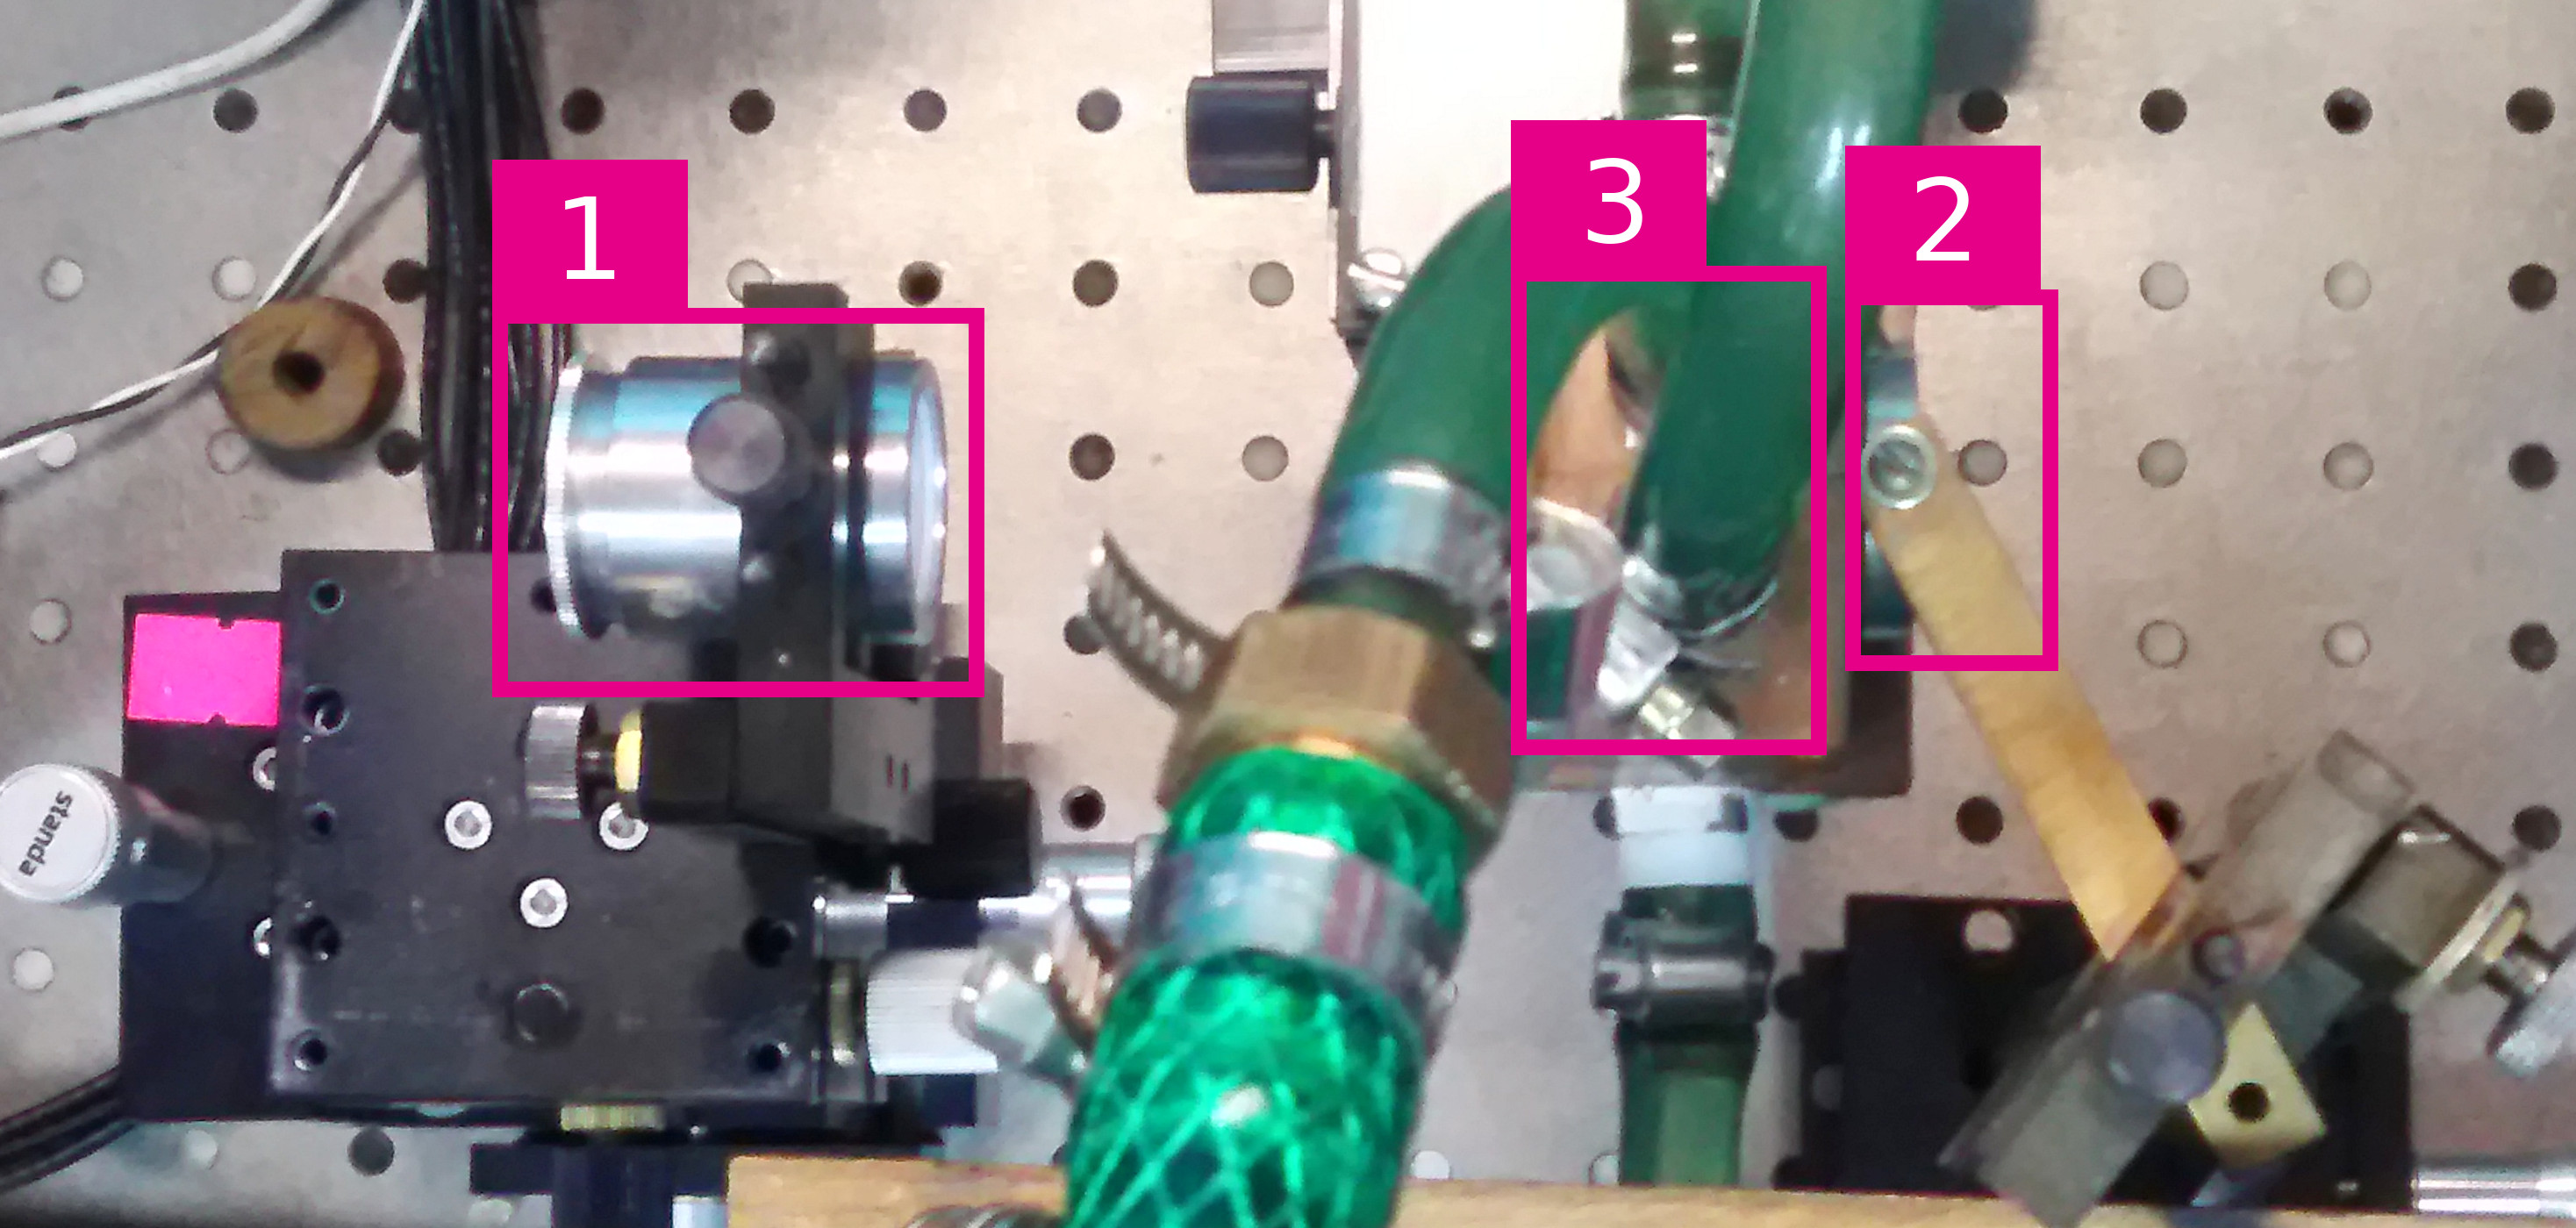
\includegraphics[width=\textwidth]{photo/s.jpg}
				\caption{Экспериментальный лазер на керамике}
			\end{figure}
		\end{column}
		% \hspace{1.6cm}
		\begin{column}{0.4\textwidth}
			\begin{figure}[tb]  
				\centering
				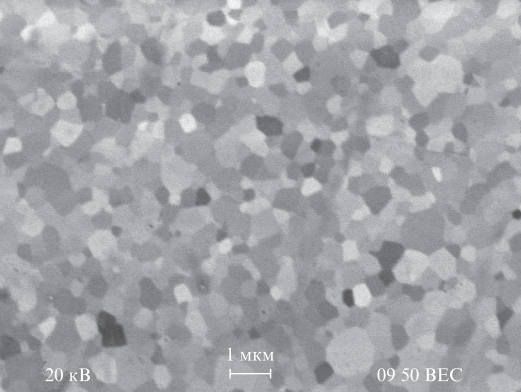
\includegraphics[width=\textwidth]{photo/ke.jpg}
				\caption{Структура керамики}
			\end{figure}
		\end{column}
	\end{columns}	
		\vspace{1em}
	\begin{columns}
		\begin{column}{0.6\textwidth}
			\textbf{1} -- выходное зеркало резонатора \\
			\textbf{2} -- входное зеркало резонатора \\
			% ,\textbf{2} -- зеркала резонатора\\ 
			\textbf{3} -- активная среда с термостабилизацией
		\end{column}
		% \hspace{1.6cm}
		\begin{column}{0.4\textwidth}
			Характерный размер зерна керамики (кристаллита) $\sim 500$ нм $\Rightarrow$ малые потери на рассеяние
		\end{column}
	\end{columns}	
\end{frame}
%%%%%%%%%%%%%%%%%%%%%%%%%%%%%%%%%%%%%%%%%%%%%%%%%%%%%%%%%%%%% 
\begin{frame}[t]
	\frametitless{Зависимость излучения лазера на керамике от тока}
		\begin{figure}[tb]
		\centering
		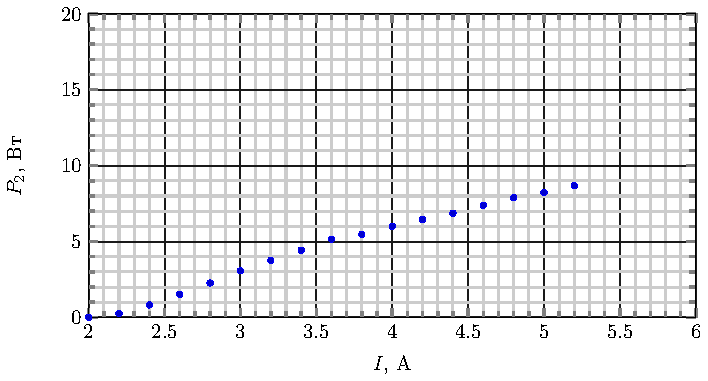
\includegraphics[height=0.85\textheight]{img/P2I2}
	\end{figure}
\end{frame}
%%%%%%%%%%%%%%%%%%%%%%%%%%%%%%%%%%%%%%%%%%%%%%%%%%%%%%%%%%%%% 
\begin{frame}[t]
	\frametitless{Настроенная мода лазера на керамике}
	\vfill
\
			\begin{figure}[h]
				\centering
				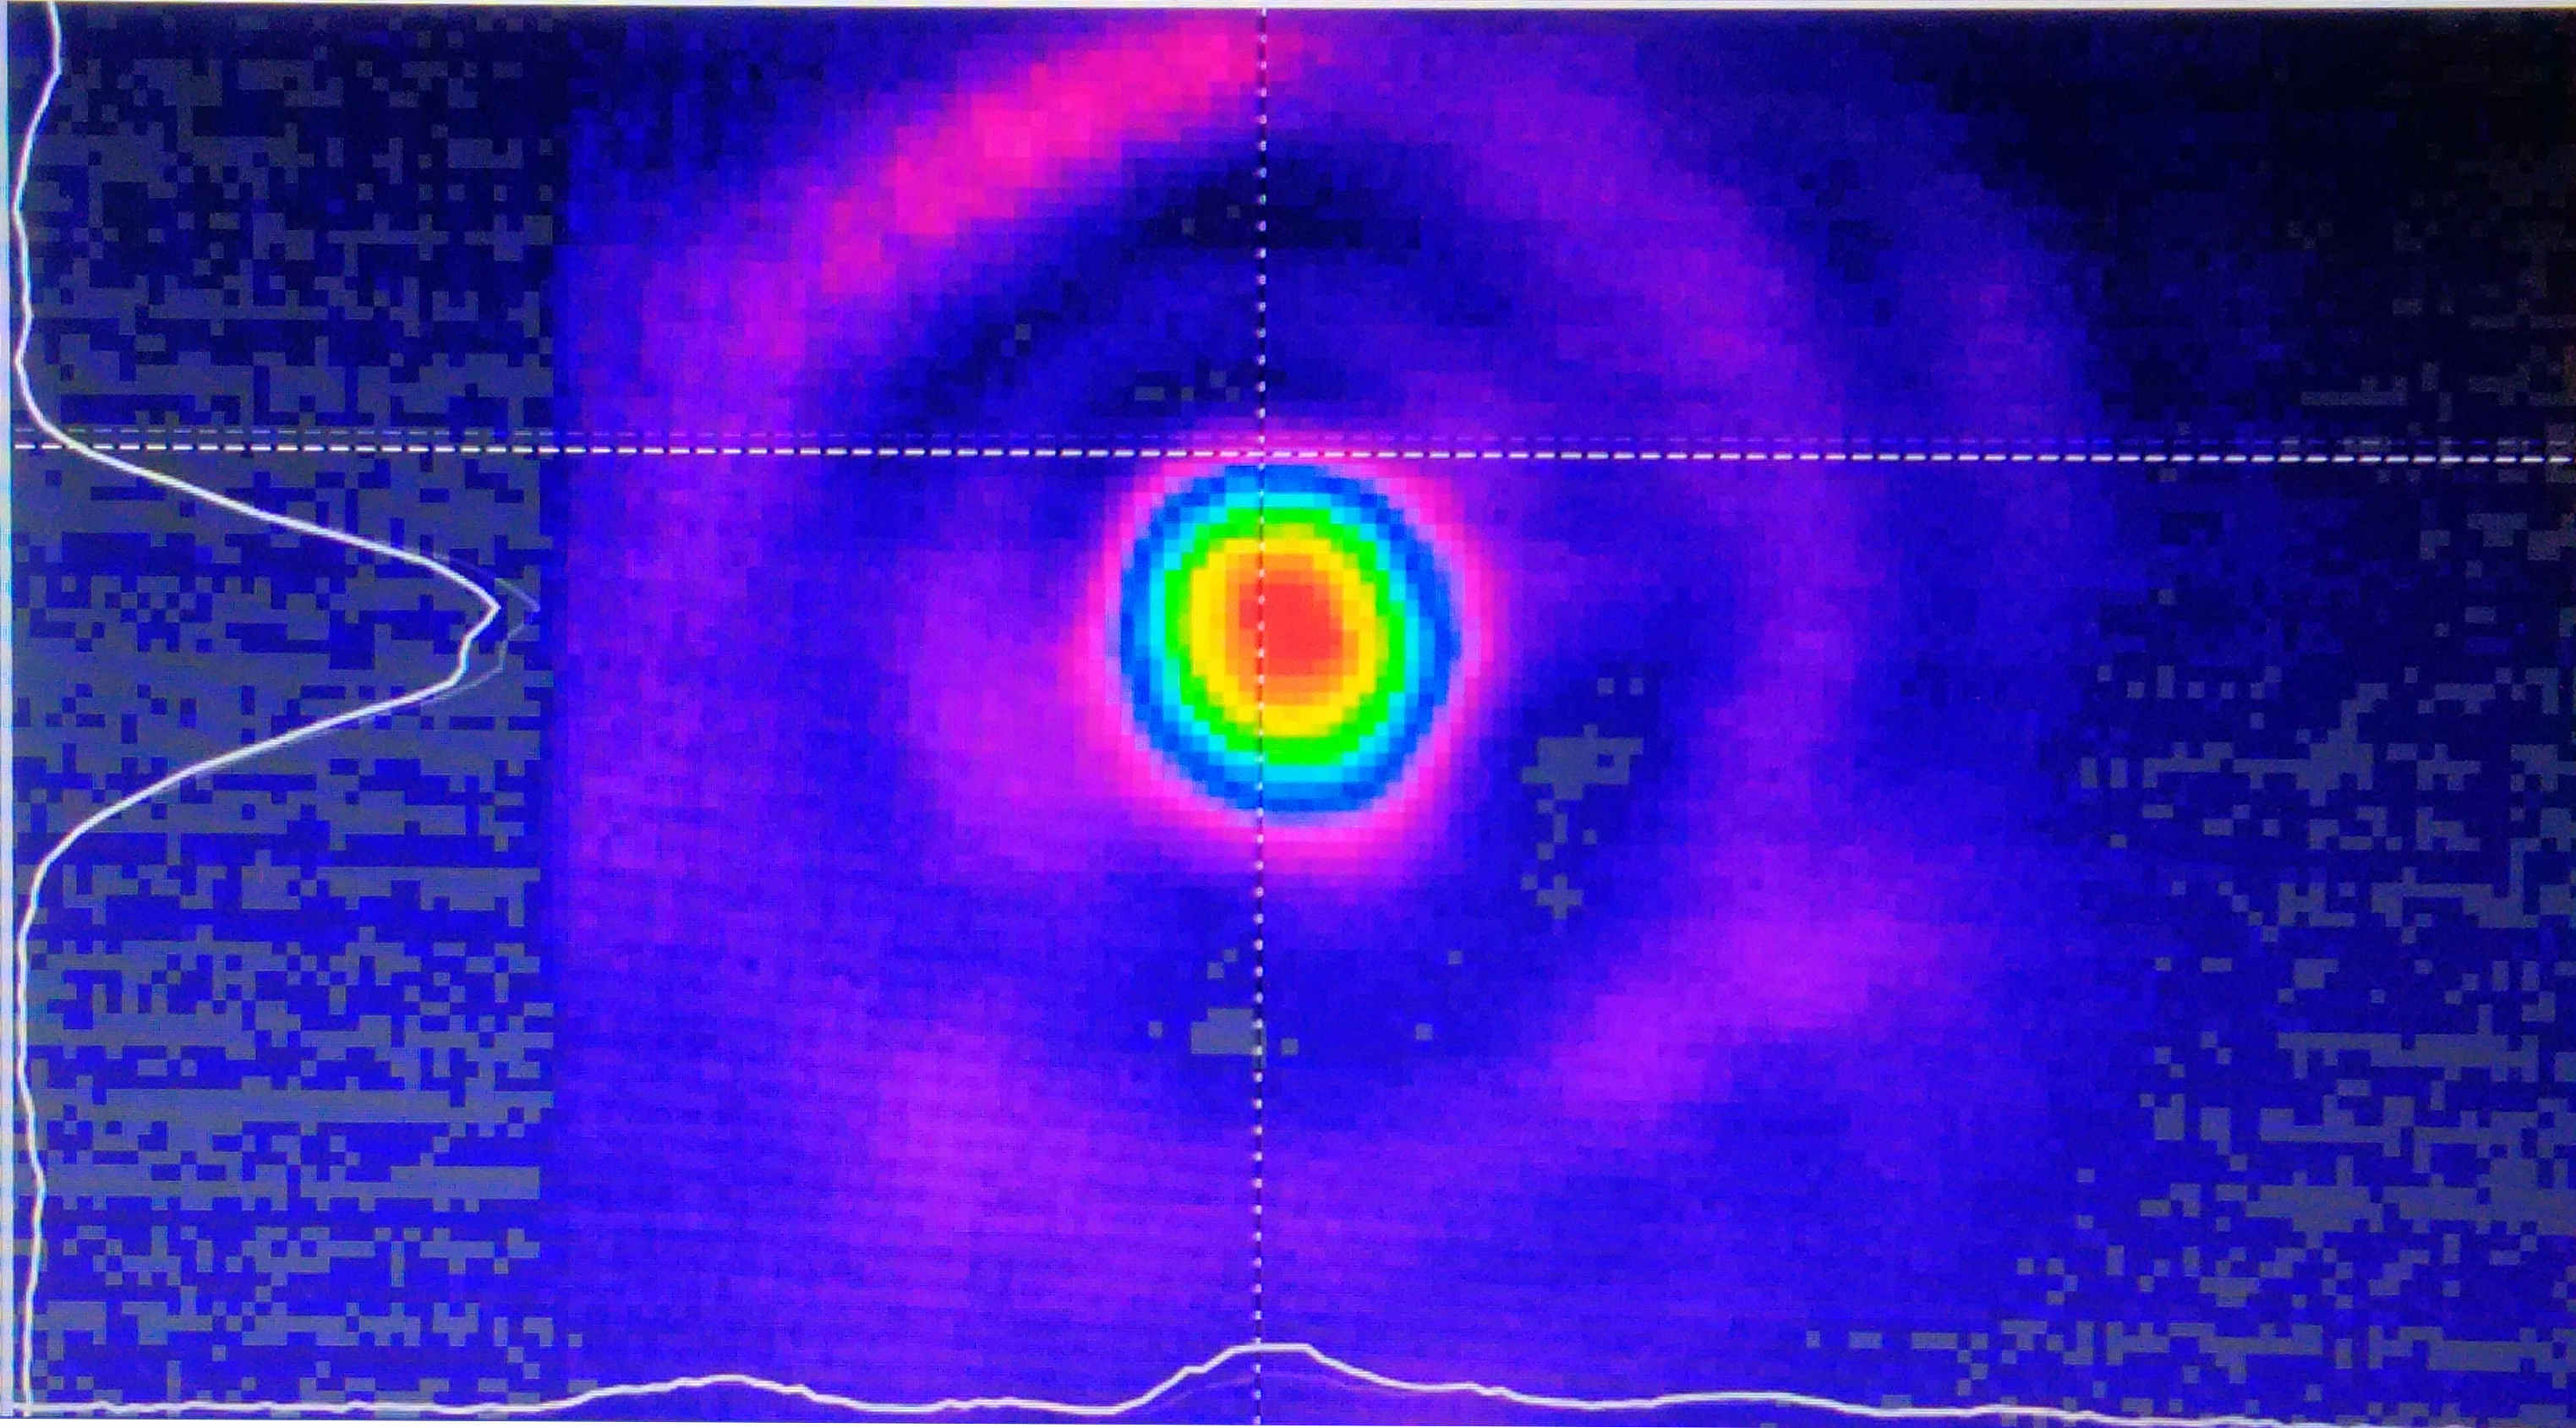
\includegraphics[width=\textwidth]{photo/light}
				\caption{Основная поперечная мода лазера на керамике}
			\end{figure}	
	\vfill
\end{frame}
%%%%%%%%%%%%%%%%%%%%%%%%%%%%%%%%%%%%%%%%%%%%%%%%%%%%%%%%%%%%% 
\begin{frame}[t]
	\frametitless{Зависимость излучения лазера на керамике от мощности накачки}
		\begin{figure}[tb]
		\centering
		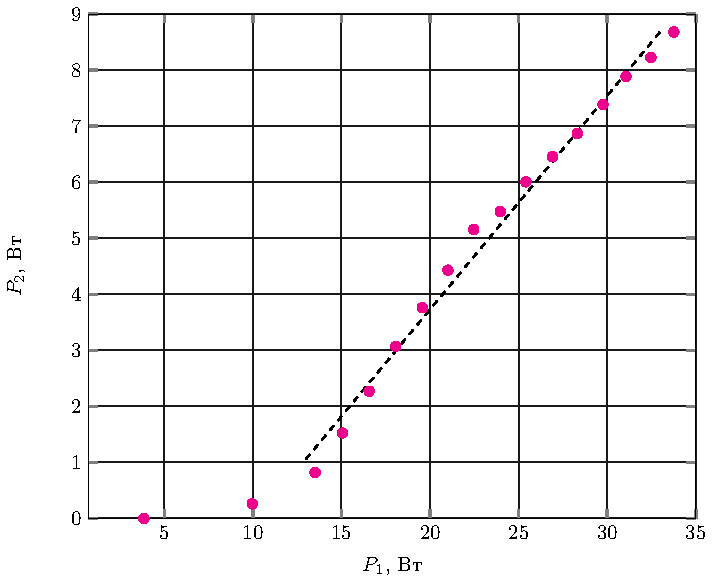
\includegraphics[width=0.73\textwidth]{img/P2P1}
	\end{figure}
\end{frame}
%%%%%%%%%%%%%%%%%%%%%%%%%%%%%%%%%%%%%%%%%%%%%%%%%%%%%%%%%%%%%
\begin{frame}
	\frametitless{Выводы}
	В данной работе были:
	\begin{enumerate}
		\item Осуществлено знакомство с принципами работы  лазера
		\item Измерена мощность волоконного лазера
		\item Проведен эксперимент по созданию лазера на керамике
		\item Измерена мощность лазера на керамике
	\end{enumerate}
\end{frame}

%%%%%%%%%%%%%%%%%%%%%%%%%%%%%%%%%%%%%%%%%%%%%%%%%%%%%%%%%%

\begin{frame}[plain]
	\vspace{4cm}
	\begin{center}
		\Huge
		Спасибо за внимание!
	\end{center}
	\vspace{2.5cm}
	\begin{center}
		\color{black!30!white}
		Презентация подготовлена в издательской \\
		системе LaTeX с использованием пакетов \\
		PGF/TikZ и Beamer
	\end{center}
\end{frame}
\end{document}